\documentclass[12pt]{article}
\usepackage[paper=a4paper,left=20mm,right=20mm,top=30mm,bottom =30mm]{geometry}
\usepackage[utf8]{inputenc}
\usepackage[T1]{fontenc}
\usepackage{stmaryrd}
\usepackage{setspace}
\usepackage{mathrsfs}
\usepackage[ngerman]{babel}
\usepackage{amssymb}
\usepackage{amsmath}
\usepackage{fancyhdr}
\usepackage[dvips,unicode,colorlinks,linkcolor=black]{hyperref} 
\usepackage{graphicx}
\usepackage{float}

\pagestyle{fancy}
\lfoot{}
\rfoot{Paul Kremser, Tobias Grussenmeyer}
\cfoot{\thepage}
\fancyhead[L]{FPI Versuch: Lange Halberwertszeiten}
\renewcommand{\headrulewidth}{0.6pt}
\renewcommand{\footrulewidth}{0.6pt}
\setlength{\headheight}{16pt}
\setlength{\parindent}{0pt}
% Für die Wahl der Schriftart
\newcommand{\changefont}[3]{
\fontfamily{#1} \fontseries{#2} \fontshape{#3} \selectfont}

\begin{document}
% keine Hurenkinder und Schusterjungen
\clubpenalty = 10000
\widowpenalty = 10000 
\displaywidowpenalty = 10000

\onehalfspacing
% Schriftart
\changefont{ptm}{m}{n} 

\begin{titlepage}
\author{Paul Kremser, Tobias Grussenmeyer}
\title{Versuch: Lange Halbwertszeiten}
\date{Versuchsdurchführung: 6. und 7. Oktober 2009} 
\maketitle
\thispagestyle{empty}
\end{titlepage}


\tableofcontents
\thispagestyle{empty}
\newpage
\pagenumbering{arabic}
\section{Überblick}
In diesem Versuch werden die Halbwertszeiten des $\alpha$-Strahlers $ ^{147}Sm$ und des $\beta$- Strahlers $^{40}K$ bestimmt. Da es sich um extrem langlebige Nuklide handelt $(T_{\frac{1}{2}} =1.06 \cdot 10^{11}$s  bzw.$1.28 \cdot 10^9$ Jahre) ist eine Beobachtung der Änderung der Impulsrate in Abhängigkeit von der Zeit nicht mehr möglich. Die Halbwertszeit $T_{\frac{1}{2}}$ lässt sich jedoch aus der spezifischen Aktivität $A_s$ bestimmen. Zur experimentellen Durchführung wird ein Methan-Durchflußzählrohr verwendet. Die radioaktiven Präparate (mit Aktivitäten < $200 Bq$) werden in ein direkt unter dem Zählrohr befindliches Probenrad eingebracht. Bei jeweils fest gewählter Hochspannung in den Plateaubereichen des Zählrohres werden die Aktivitäten der Präparate gemessen. Aus dem Zerfallsgesetz $A = ln(2) \frac{N}{T_{\frac{1}{2}}}$ kann bei bekannter Zahl der zerfallenden Atome N und nach einer Bestimmung der Aktivität A die Halbwertszeit $T_{\frac{1}{2}}$ berechnet werden. Zur Bestimmung der absoluten, d.h. durch Effekte wie Selbstabsorption und Rückstreuung nicht verfälschten, Aktivität aus den tatsächlich gemessenen Aktivitäten werden verschiedenen Methoden verwendet: Die Aktivität des $\alpha$-Strahlers Samarium wird
unter Ausnutzung der konstanten Reichweite der Strahlung und der bekannten Oberfläche des Präparats korrigiert. Beim $\beta$-Strahler Kalium wird die Massenabhängigkeit der beobachteten Aktivität ausgenutzt.


\section{Aufgabenstellung}
In diesem Versuch werden die Halbwertszeiten des $\alpha$-Strahlers $^{147}Sm$ und des $\beta$-Strahlers $^{40}K$ bestimmt. Da es sich dabei um sehr langlebige Nuklide handelt, ist eine direkte Bestimmung der Halbwertszeit aus der Beobachtung der Zeitabhängigkeit der Impulsrate nicht mehr möglich. Stattdessen werden die Halbwertszeiten aus der Aktivität der Präparate bestimmt. Bestimmung der Halbwertszeit von $^{147}Sm$ ($\alpha$-Zerfall)
\begin{enumerate}
 \item Bestimmung der Halbwertszeit von $^{147}Sm$ ($\alpha$-Zerfall)
\begin{itemize}
 \item Aufnahme der Zählrohrcharakteristik mit einem Natururan-Präparat
 \item Wahl des Arbeitspunktes auf dem $\alpha$-Plateau
 \item Messung des Nulleffekts
 \item Ermittlung der Aktivität des Samarium-Präparats (raumwinkelabhängige Messung)
\end{itemize}
\item Bestimmung der Halbwertszeit von $^{40}K$ ($\beta ^-$-Zerfall, EC)
\begin{itemize}
\item Aufnahme des $\beta$-Plateaus mit dem Kalium Präparat
\item Wahl des Arbeitspunktes auf dem $\beta$-Plateau
\item Messung des Nulleffekts
\item Ermittlung der spezifischen Aktivität des Kalium-Präparats (massenabhängige Messung)
\end{itemize}
\end{enumerate}

\section{Theoretische Grundlagen}
\subsection{Zerfallsgesetz und Aktivität}
Beim radioaktiven Zerfall ist die Wahrscheinlichkeit das ein Teilchen in einem Zeitintervall $dt$ zerfällt bestimmt durch die \textit{Zerfallskonstente} $\lambda$. Diese Wahrscheinlichkeit beträgt $\lambda dt$, bei $N$ Teilchen die zerfallen können zerfallen also im nächsten Zeitintervall $N\lambda dt$ Teilchen. Daraus ergibt sich das Zerfallsgesetz zu
\begin{align}
 N(t) = \int \limits_{0} \limits^{t} dN = \int \limits_{0} \limits^{t} - \lambda N dt = N_0 e^{-\lambda t}
\end{align}

wobei $N_0$ die zerfallsfähigen Teilchen zur Zeit $t=0$ angibt.\\
Die \textit{Halbwertszeit} $T_{\frac{1}{2}}$ eines Stoffes gibt an wie lange es dauert bis die Hälfte der Teilchen zerfallen sind. Es folgt also
\begin{align}
N(T_{\frac{1}{2}} = \frac{1}{2} N_0 = N_0 e^{ -\lambda T_{\frac{1}{2}}} \Rightarrow T_{\frac{1}{2}} = \frac{ln(2)}{\lambda}
\end{align}

Unter der \textit{Aktivität} $A$ versteht man die Anzahl der zerfallenden Teiclhen pro Zeit also 
\begin{align}
 A = -\frac{dN}{dt} = \lambda N
\end{align}
Unsere Stoffe haben im Überblick beschrieben sehr Lange Halbwertszeiten, so dass man die Aktivität hier durchaus als konstant annehmen kann. Somit folgt für unsere Halbwertszeit:
\begin{align}
 T_{\frac{1}{2}} = \frac{N ln(2)}{A}
\end{align}

\subsection{Zerfallsarten}

Beim Radioaktiven Zerfall gibt es unterschiedliche Prozesse bei der verschiedene Zerfälle stattfinden. Dabei werden auch unterschiedliche Arten Radioaktiver Strahlung emittiert.

\begin{itemize}
 \item $\alpha$ Zerfall
Ein angeregte Atom geht unter aussendung eines Helium-Kerns in einen stabileren Zustand über. Alle $\alpha$-Teilchen eines bestimmten Übergangs weisen dieselbe Energie auf, da die beteiligten Niveaus diskret sind und nur ein Teilchen emittiert wird. Die Zerfallsgleichung für $^{147}Sm$ lautet:
\begin{align}
 \notag ^{148}_{62}Sm \longrightarrow ^{144}_{60}Nd + ^4_2He
\end{align}


\end{itemize}


\section{Versuchsaufbau}

\section{Durchführung}

\section{Auswertung}
\subsection{Zählrohrcharakteristik mit Uran}
Anfangs versuchten wir Einstellungen der Elektronik zu finden bei denen die Zählrate maximal ist, jedoch war darauf zu achten dass keine Teilchen doppelt
gezählt werden. Wir entschieden uns für folgende Einstellungen:
\begin{itemize}
 \item Verstärker: Gain 7,20; Coarse Gain 20; Shaping Time 1$\mu s$
 \item Timing SCA: low level 3,0; high level 10,0; delay 1,0
 \item Gate: delay 1,0 $\cdot$ 1,1$\mu s$
\end{itemize}

Zu Begin machten wir eine Messung mit einem Uranpräparat um die Charakteristik des Zählrohrs kennen zu lernen.
Hierzu gingen wir in 100$V$ Schritten von 1000$V$ bis 4000$V$ mit einer jeweiligen Messdauer von 50$s$.
Außerdem machten wir mit den selben Einstellungen eine Untergrundmessung von von 1600 bis 4000$V$ mit jeweils 100$s$
Messdauer und verwendeten diese um die Zählrohrcharakteristik zu korrigieren.

Der Fehler auf die Zählrate berechnet sich dann wie folgt:
\begin{align}
 s_n = \frac{s_N}{t} = \frac{\sqrt{N}}{t} = \frac{\sqrt{n~t}}{t} = \sqrt{\frac{n}{t}}
\end{align}

Mit Gesamtanzahl der Counts $N$, Fehler auf diese $s_N$, Zählrate $n$ und jeweilige Messdauer $t$. Wobei wir den Fehler auf die Messdauer
vernachlässigen.


\begin{figure}[H]  
\centering
\includegraphics[width=0.9\linewidth]{pictures/char_uran.eps}
\caption{Zählrohrcharakteristik mit Uran}
\end{figure}


\subsection{Halbwertszeit von Samarium}
Zuerst nahmen wir das $\alpha$-Plateau auf. Hierfür orientierten wir uns an der mit Uran aufgenommenen Charakteristik (1800-3400$V$).
Diese Messung geschah mit den selben Einstellungen wie die mit Uran und kann daher mit der selben Untergrundmessung korrigiert werden.

\begin{figure}[H]  
\centering
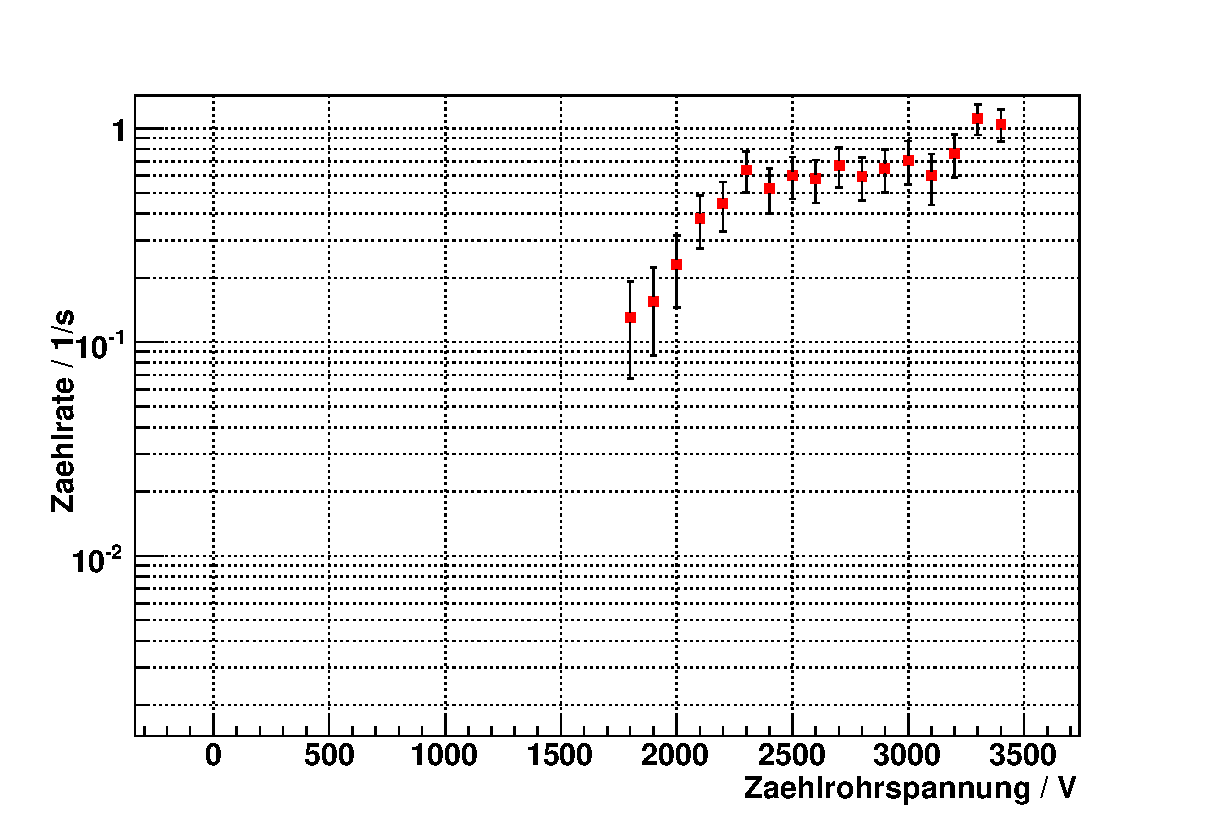
\includegraphics[width=0.9\linewidth]{pictures/char_sam.eps}
\caption{Zählrohrcharakteristik mit Samarium}
\end{figure}

Aus der Messung bestimmten wir demn Arbeitspunkt bei 2600$V$ und konnten mit der dort gemessenen Rate die benötigte Messzeit um den Messfehler unter
2\% zu bekommen berechnen (4300$s$). Ebenso konnten wir die Messzeit für die Untergrundmessung berechnen um einen Beitrag zum Fehler auf die Rate
von $1/3$ zu erhalten (3000$s$).

Die tatsächliche Rate $n$ setzt sich dann aus gemessener Rate $n*$ und Untergrund $u$ zusammen: $n = n* - u$. Wenn man auch hier wieder den Fehler auf
die Zeit vernachlässigt, erhält man für den Fehler:
\begin{align}
 s_n = \sqrt{s_{n*}^2 + s_u^2} = \sqrt{\frac{n*}{t} + \frac{u}{t}} = 0,01 s^{-1}
\end{align}

Um den durchmesser der Probe zu bestimmen maßen wir diesen abwechselnd mit einer Schiebelehre und erhielten dabei zweimal 2,905 und achtmal 2,900.
Daraus ergibt sich ein Durchmesser von $d = (2,901~ \pm~ 0,0016)cm$ wenn man 0,005$cm$ als Ablesefehler annimmt. Was wiederum eine Fläche von
$F = \frac{\pi}{4}~d^2 = 6,606 cm^2$ mit einem Fehler von
\begin{align}
 s_F = \sqrt{\left(\frac{\partial F}{\partial d}\right)^2~s_d^2} = \frac{\pi}{2}~d~s_d = 0,007 cm^2
\end{align}
ergibt.

Mit Rate und Fläche lässt sich nun die Halbwertszeit bestimmen:
\begin{align}
 t_{\frac{1}{2}} = \frac{R~\rho~ln 2 ~ N_A ~ h_{rel} ~ F}{2~m_{r,Sm_2O_3}~~n}
\end{align}

mit dem Fehler:
\begin{align}
 s_{t_{\frac{1}{2}}} = \sqrt{\left(\frac{s_F}{F}\right)^2 + \left(\frac{s_n}{n}\right)^2}~\cdot~t_{\frac{1}{2}}
\end{align}

Als Ergebins für die Halbwertszeit von $^{147}Sm$ erhielten wir:
\begin{align*}
 t_{\frac{1}{2}} = (2,1518~\pm~0,0643)~\cdot~10^11~a
\end{align*}


\begin{figure}[H]  
\centering
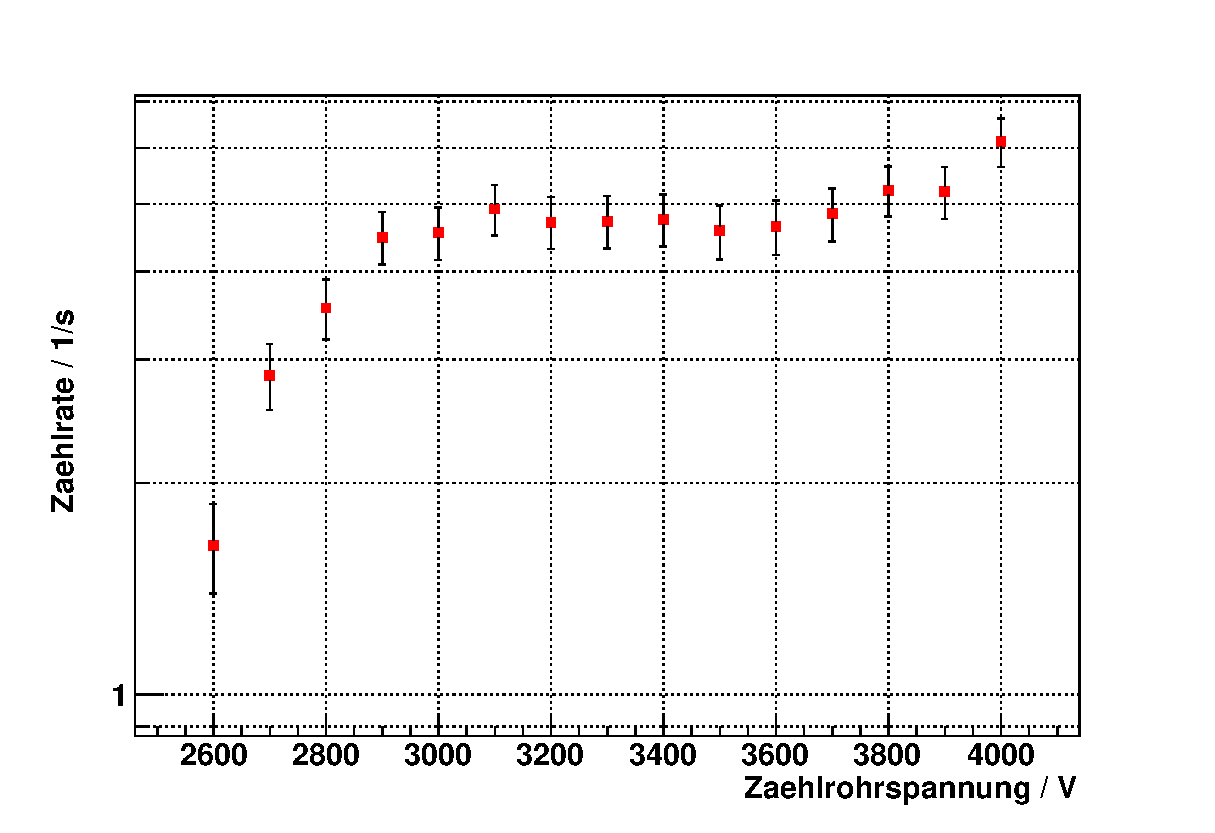
\includegraphics[width=0.9\linewidth]{pictures/char_kalium.eps}
\caption{Zählrohrcharakteristik mit Kalium}
\end{figure}

\begin{figure}[H]  
\centering
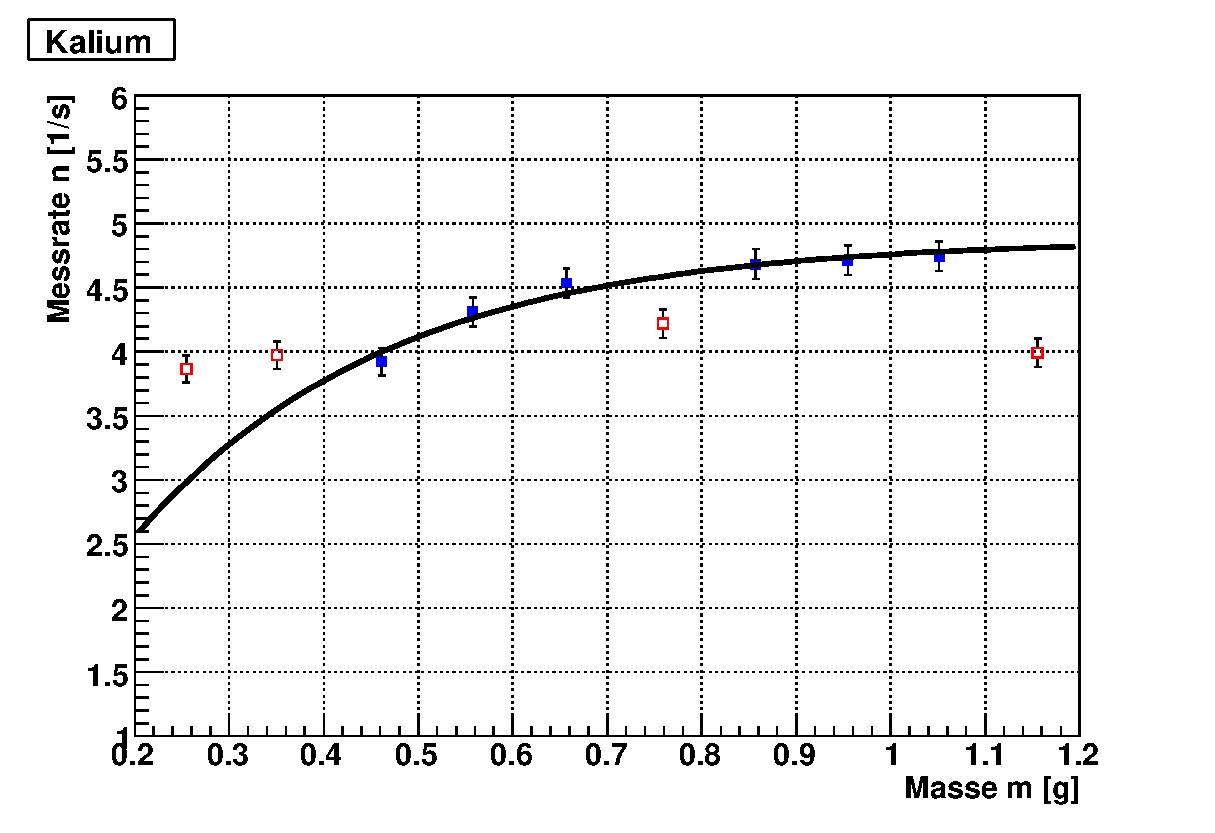
\includegraphics[width=0.9\linewidth]{pictures/kalium.eps}
\caption{Massenabhängigkeit mit Kalium}
\end{figure}

\section{Zusammenfassung}

\end{document}
